%%%%%%%%%%%%%%%%%%%%%%%%%%%%%%%%%%%%%%%%%%%%%%%%%%%%%%%%%%%%%%%%%%%%%%%%%%%%%%%%
%%% Material
%%%%%%%%%%%%%%%%%%%%%%%%%%%%%%%%%%%%%%%%%%%%%%%%%%%%%%%%%%%%%%%%%%%%%%%%%%%%%%%%

\clearpage
\section{Project and materials}
\label{sec:materials}

In this section I will describe the project plan starting with describing the existing systems that I had to integrate with.
Next, I will describe the data that was available to be used for the project. 
Lastly, I will describe the project schedule.

\subsection{Existing systems}

The project was to be integrated on top of existing diagnostics systems to save time and to improve the overall user experience by leveraging the system they were already familiar with.
The store has an internal monitoring tool called \textbf{Jury} for the store engineers and other users to visualize details and relationships of the products and publishers in the store.
Jury implements a user interface to query the production database for products, publishers, and events.
Jury also handles authentication, authorization, and permissions.
This is needed to preserve the confidentiality of private information.

Jury includes a textual query language to filter and search the database.
The query language allows the users to search for the information that they are interested in.
The queries can be saved for later use. 
The saved queries can be used as shortcuts or ``dashboards'' for the users.
For example, a user can save a query that searches for new products published within the last 24 hours.
This query can then be used by the user to periodically check the new products.

A major goal for this project was to make use of the existing query system as much as possible.
This way the benefits, like user-made views and integration with the saved queries, could be re-used.
The statistics and any real-time visualizations should use the query system to retrieve the events.
When retrieving the events, the user's permissions need to be taken into account to preserve confidentiality.

\subsubsection{Azure ML}

\textbf{Azure ML} (publicly available at \cite{azuremlpub}) is a cloud service that offers machine learning capabilities on demand. 
They offer ready-made machine learning models in the cloud for anyone to use.
They also allow the user to provide their own code or models.
One of the major features Azure ML offers is a visual interface for machine learning called the ``Machine Learning Studio'' \cite{azureml}.
This interface allows the user to set up the data flow of their machine learning solution visually with a ''drag and drop'' model and then execute it in the cloud.

I chose Azure ML for my solution because of the accessibility, quick setup, and the multitude of ``off the shelf'' models offered.
With Azure ML I was able to take the data I had and start training models quickly without setting up anything on my local machine.

\subsection{Data}
% description of event hub
The data used by the project is a list of events. The events are the log entries generated by the distributed processes of the store ingestion/publishing system. Each store system creates events and sends them through an \textit{Azure Event Hub}. 
For example, there could be an ``Screenshot Upload'' event notifying that the application screenshots were successfully uploaded to a server.
Another example could be a ``Complete Publish'' event that signals that the application has finished the publishing process completely.
Azure Event Hubs are a shared event streaming service that works as a platform-independent ``front door'' for all the events \cite{eventhubs}, 
which all the events go through before being read.

The event hub is divided into several separate partitions to improve availability \cite{eventhubavail}.
Furthermore, separate partitions allow for concurrent reads of events to improve throughput.
All the processors of the store systems broadcast events into a common Event Hub.
The events are then read and processed by Jury and stored in a SQL database.
My project did not concern the event hub, instead I only read the events as they appeared in the database.

% specific description of events and how they are stored
Each event consists of a \textbf{timestamp} and some metadata. 
The event also has a \textbf{submission identifier} which identifies the trace that the event belongs to.
All events with the same submission identifiers belong to a single trace.
The event timestamp describes the exact time the event happened. 
There are also two reference fields (foreign keys) referencing the \textbf{product} and the \textbf{publisher} that the event belongs to. 
Since these references are not used in this thesis, they can be seen simply as integer type identifier fields.
In addition to these, the three other fields relevant in this research are textual (string-type) fields \textbf{Source}, \textbf{Subsource}, and \textbf{Status}.
The event type is described in table \ref{tab:event}.

\begin{table}[htb]
\begin{center}
\begin{tabular}{| c |}
\hline
\textbf{Event} \\
\hline
SubmissionId : long integer\\
ProductId : long integer\\
PublisherId : long integer\\
Timestamp : DateTime\\
Source : string\\
Subsource : string\\
Status : string\\
\hline
\end{tabular}
\end{center}
\caption{Event and its fields}
\label{tab:event}
\end{table}

The Source field identifies the event source system, whereas the Subsource identifies the exact processor step withing that system. 
For example, for an event related to uploading images to a server during the publishing phase, the Source field could have the value ``Publishing'' and the Subsource a value of ``Upload Images''.
Thus, the Source--Subsource pair is enough to identify the exact step of the workflow which generated the event. 
The Status field contains a string describing the status of the step, such as ``Completed'', ``In progress'' or ``Failed''. 
This field can be used to reason about the duration of the events and to determine whether the event is \emph{final}. 
A final-status event means that the processor has completed the activity and will not be sending further events for the activity in question.
For example, events marked with ``Completed'' or ``Failed'' status are final.
In contrast, events with an ``In progress'' status are \emph{non-final}.
These events are fired to show that a long-running activity has been started, is still running, and hasn't failed.
An ``In progress'' will eventually be followed by a final event such as ``Completed'' or ``Failed'' with the same Source and Subsource.
The common statuses are listed in table \ref{tab:statuses}.

% methods explaining splitting and grouping of traces
An arbitrary set of events can be grouped into traces by the submission identifier field. 
Within the trace each individual step can then be identified by the Source--Subsource pair.
In a valid trace there should only be a single final event for each distinct Source--Subsource pair.

\begin{table}[htb]
\begin{center}
\begin{tabularx}{\linewidth}{| l | c | X | }
\hline
\textbf{Status} & \textbf{Final} & \textbf{Meaning} \\
\hline
Completed   & Yes & The activity was completed successfully. \\
\hline
Skipped     & Yes & The activity was not needed for this submission and was skipped. \\
\hline
Failed      & Yes & The activity was completed with an error. The activity may be retried or the whole workflow may be stopped. \\
\hline
In progress & No  & The activity has been started, is running, and will finish later. \\
\hline
\end{tabularx}
\end{center}
\caption{The common values of the status field of events}
\label{tab:statuses}
\end{table}

\subsubsection{Challenges found in the production data}
\label{sec:datachallenges}

In section \ref{sec:eventtheory} we considered the event log to be a totally ordered flat log. 
In this theoretical log each event would have a clear case identifier and its location within the flat log would correspond to the real world ordering of the events.
In theory, this case identifier and the log order can be used to split the log into traces and further order the events in each trace.
However, the production data proved to be more complex than that. 

% event hub ordering
As mentioned earlier, the event hub processors work in several partitions to improve availability.
Within a partition, the order of events is guaranteed to be stable with regards to events arriving to the event hub. 
However, there is no guarantee on the interleaving of the parallel processing of the partitions.
When the events are processed by Jury, the order between the partitions may be different compared to the event arrival order. 
Thus, the event order (the row number) in the SQL database should not be fully trusted.
Furthermore, network issues or other delays can affect event ordering. 
To combat this, each event is marked with a timestamp by the sender. 
With the timestamp the estimated ordering of events can be rebuilt when they are read from the SQL database.

% clock skew between different systems
However, the events are generated by a separate systems in parallel.
Each of these systems depends on its own hardware clock, and the clock synchronization between the systems is not guaranteed to be exact. 
This means that even the timestamps may include an unknown error for up to several minutes.
Furthermore, some events may be lost because of bugs, unhandled exceptions, or outages in the system.
This means that ordering the events by timestamp includes random noise, which needs to be considered.

% Incomplete traces in the chosen ''slice'' (events missing from beginning/end)
Another aspect to note is that when the event log data is used, the data being analyzed is always a ``slice'' of the full event log.
This means that it contains events from a time slice starting at some time instance $t_s$ and ending at some later time $t_e$, as illustrated in figure \ref{fig:timeslice}. 
All events between these times are considered. 
A common use case would be to inspect the past 24 hours of events. 
In this case $t_e$ is the current time, and $t_s$ is 24 hours earlier than the current time. 
This results in the time slice containing a large amount of events that belong to a trace that started before $t_s$ (case \textit{b} in figure \ref{fig:timeslice}).
The result also contains traces that have yet to be completed (cases \textit{c} and \textit{d} in figure \ref{fig:timeslice}).
These traces should be removed, since the beginning or the end of the trace is missing.
Classifying a trace as anomalous like this requires an \emph{appropriate model} \cite{bezerra2009anomaly},
meaning some prior understanding is needed on how to discover whether a trace is invalid.

\begin{figure}[htb]
\centering 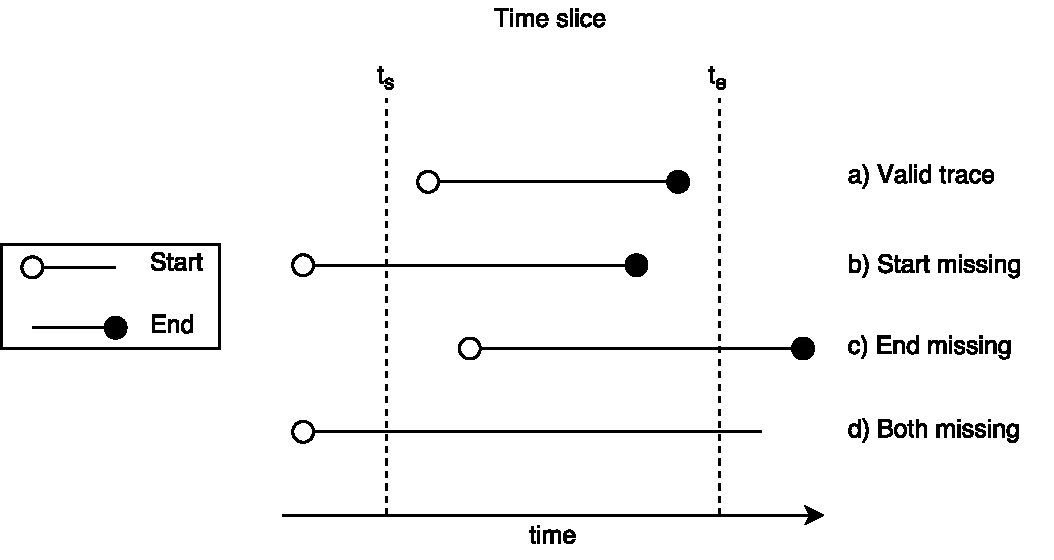
\includegraphics[width=0.8\linewidth]{gfx/figures/timeslice.pdf}
\caption{Time slice and validity of traces}
\label{fig:timeslice}
\end{figure}

% resubmissions
When talking about the process mining theory (see section \ref{sec:eventtheory}) it was assumed that each trace can be uniquely identified.
This means splitting the traces from the flat event log and identifying the individual cases.
For this specific system, each submission of a product has a unique \emph{submission identifier} (submission ID).
This ID can be used to uniquely identify a trace.
However, in practice this proved more complicated.
Sometimes the application submission can be \textit{re-submitted} into the store.
This is commonly done if some part of the workflow fails to complete.
The events in such a re-submission will have the same submission ID as the original submission.
This leads to a situation where the trace seems to restart from the beginning or from a different step and continue. 
These cases should be identified as anomalous. 
In the case of real-time data, only the latest submission for each ID should be considered, since the earlier submissions are rarely relevant to the user.

Another big challenge comes from the real-time characteristics of the data. 
Because of agile practices and continuous delivery, the store systems are under constant change. 
This means that the underlying process model can change any time.
The process model generated a day before may not reflect the current state anymore. 
The system should be flexible and should adapt to any changes in the underlying models.

% invalid states
Furthermore, the production data will also include traces that have failures or phases that are in progress.
A trace with failed or erroneous steps should be considered anomalous, since a workflow is not guaranteed to progress normally after an error. 
Similarly, the traces include events that do not describe a final state, but only broadcast status. 
The most common type of event like this events with an ``In progress'' status.
If an event is non-final, it means that the same process is still expected to fire a final event afterwards.
These events should be handled differently in the modeling phase.

All these characteristics require that the system uses some kind of pre-processing method that takes the slice of the real-world data and outputs an ordered and grouped set of traces with the anomalous traces removed.

\subsection{Project timeline}
\label{sec:timeline}
% description of research timeline
% weekly meetings with manager, PM
I started preparing for the project in late 2016.
The project started in Redmond, Washington, USA in early January 2017.
While the main goal of the project was established early, the details needed some research. 
For this reason, an iterative process was set up.
I held weekly meetings with my manager, as well as weekly project meetings together with my advisors and the team program manager. 
In addition, at the midway point I held three presentations to people from the different user groups to find more requirements and to get feedback. Because of this, the project was divided in two iterations.
The weekly meetings were carried out through both iterations.
The complete timeline of the project can be seen in figure \ref{fig:projecttimeline}.

\begin{figure}[htb]
\centering 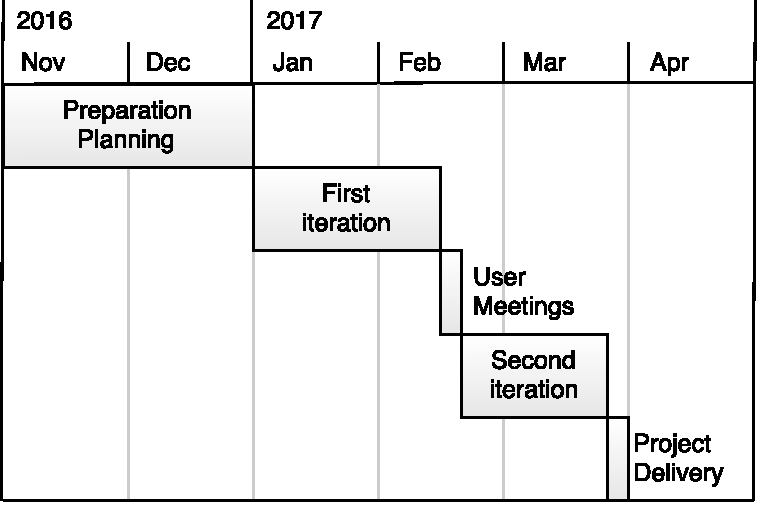
\includegraphics[width=0.7\linewidth]{gfx/figures/projecttimeline.pdf}
\caption{Project timeline}
\label{fig:projecttimeline}
\end{figure}

% - first iteration: supporting work, backend, graphing, initial UI
%   - explorative prototypes
%   - two UI proposals, graph and timeline
I started the first iteration by building a prototype using a small test dataset of events exported from the database. The purpose of the prototype was to explore the graph generation algorithms and to build a proof of concept. 
After the prototype was validated by the team I integrated it with the Jury system. 
I built two user interface proposals based on different types of presentation. The first one showed a directed graph describing the workflow model. The second interface showed the events on a scrollable timeline.
See section \ref{sec:userinterface} for the detailed descriptions of these views.

% - user meetings (brownbag, 3pp)
After the first iteration I held three presentations, two of which included a feedback session with exploration for use cases. The first presentation was an open one to the higher management and the other teams. The second presentation was with the release managers to get feedback from them and to find more requirements. The third was a ``brown bag'' type of open meeting with other team members who interact with the Jury system.
In these meetings I validated my prototype designs and collected feedback about the user interface.
In the meetings the timeline view was seen more useful for most user groups.
The only exception was the engineers who saw the graph view more useful for debugging.

% - second iteration: user interface work, features to fit needs
%   - machine learning exploration
%   - graphing accuracy exploration (alt graph)
In the second iteration I spent more effort on the user interface, based on the meetings.
I experimented with machine learning models and the process discovery algorithm.
I also worked with the team to integrate the graphs with the email notification system in Jury so they could be used to send emails about delays observed in the system. 
By the end of the second iteration the project was fully integrated with Jury and was delivered to the users.